\documentclass[11pt]{article}
\usepackage[margin=1in]{geometry}
\usepackage{amsfonts, amsmath, amssymb}
\usepackage[none]{hyphenat}
\usepackage{fancyhdr}
\usepackage{graphicx}
\usepackage{float}
\usepackage[nottoc, notlot, notlof]{tocbibind}
\usepackage{hyperref}

\pagestyle{fancy}
\fancyhead{}
\fancyfoot{}
\fancyhead[L]{\slshape \MakeUppercase{Report}}
\fancyhead[R]{\slshape Erik Davino Vincent}
\fancyfoot[C]{\thepage}

\setlength{\parindent}{4em}
\setlength{\parskip}{1em}
\renewcommand{\baselinestretch}{1}

\begin{document}

\begin{titlepage}
\begin{center}
\vspace{1cm}
\Large{\textbf{ }}\\
\vfill
\line(1,0){400}\\[1mm]
\huge{\textbf{iFood - Data Analysis Case}}\\[3mm]
\Large{\textbf{- Report -}}\\[1mm]
\line(1,0){400}\\
\vfill
By Erik Davino Vincent\\
\today\\

\end{center}
\end{titlepage}

\tableofcontents
\thispagestyle{empty}
\clearpage

\setcounter{page}{1}

\section{Introduction}

Key Objectives:
\begin{itemize}
\item Explore the data. Provide insights, define cause and effect. Provide a better understanding of the characteristic features of respondents;
\item Propose and describe a customer segmentation based on customers behaviors;
\item Create a predictive model which allows the company to maximize the profit of the next marketing campaign.
\end{itemize}

\subsection{Mock Case}

The objective of the team is to build a predictive model that will produce the highest profit for the next direct marketing campaign, scheduled for the next month. The new campaign, sixth, aims at selling a new gadget to the Customer Database. To build the model, a pilot campaign involving
2.240 customers was carried out. The customers were selected at random and contacted by phone regarding the acquisition of the gadget. During the following months, customers who bought the offer were properly labeled. The total cost of the sample campaign was 6.720MU and the revenue generated by the customers who accepted the offer was 3.674MU. Globally the campaign had a profit of -3.046MU. The success rate of the campaign was 15$\%$. The objective is of the team is to develop a model that predicts customer behavior and to apply it to the rest of the customer base. Hopefully the model will allow the company to cherry pick the customers that are most likely to purchase the offer while leaving out the non-respondents, making the next campaign highly profitable. Moreover, other than maximizing the profit of the campaign, the CMO is interested in understanding to study the characteristic features of those customers who are willing to buy the gadget.

\section{Analysis of the dataset}

\subsection{Dataset Analysis}

As a first step, we opened the dataset to see what the data looked like.
There was some missing informations on the income column, which needed to be filled in. In the marital status column, there were some categories that didn't make any sense, such as 'YOLO' and 'Absurd', and some categories that were equivalent, e.g. 'Together' and 'Married' or 'Alone' and 'Single'.\\

The date of enrollment column was in a datetime format, so we transformed it to integer values in Excel.\\

A dataset with reduced dimension can be vizualized with PCA here (\ref{PCA})

\subsection{Dataset Preprocessing}

Before going forward with the analysis, it is necessary to preprocess the data, so that it can be better interpreted by the algorithms.\\

During the preprocessing we made changes to the Income data column, to the YearBirth data column, and to the categorical data column MaritalStatus.\\

For the, assuming that the mean is a good estimator for a person's yearly income and considering that only 23 out of 2240 users didn't have this information filled in, we filled in the blanks of Income with the mean.\\

The YearBirth column was clipped for a minimum of 1920, since there were some unlikely values, lower than 1900.\\

Finally, in the MaritalStatus column, the 'YOLO', and 'Alone' categories were changed to 'Single' and the 'Together' and 'Absurd' ones were changed to 'Married'.\\

\subsection{Initial Analysis}

The initial analysis is very simple - it is the summary information of the features; it serves to get a more general insight on the data, and was useful for finding out the weird categories and outliers. The tables can be seen in (\ref{Tables}).\\

From these we are able to conclude that most of the company users are undergraduation, married and on average have a monthly income of around 4300.\\

There is also some insight on the recency; the average user purchases something with the company's service once every month and a half.
Also, most people don't accept any campaign offer.

\section{Secondary Analysis}

For a second approach we will be using a correlation matrix of the features, to see what is possible to infer about the users in general and about the probability of them accepting the campaing offer.\\

\begin{figure}[H]
\centering
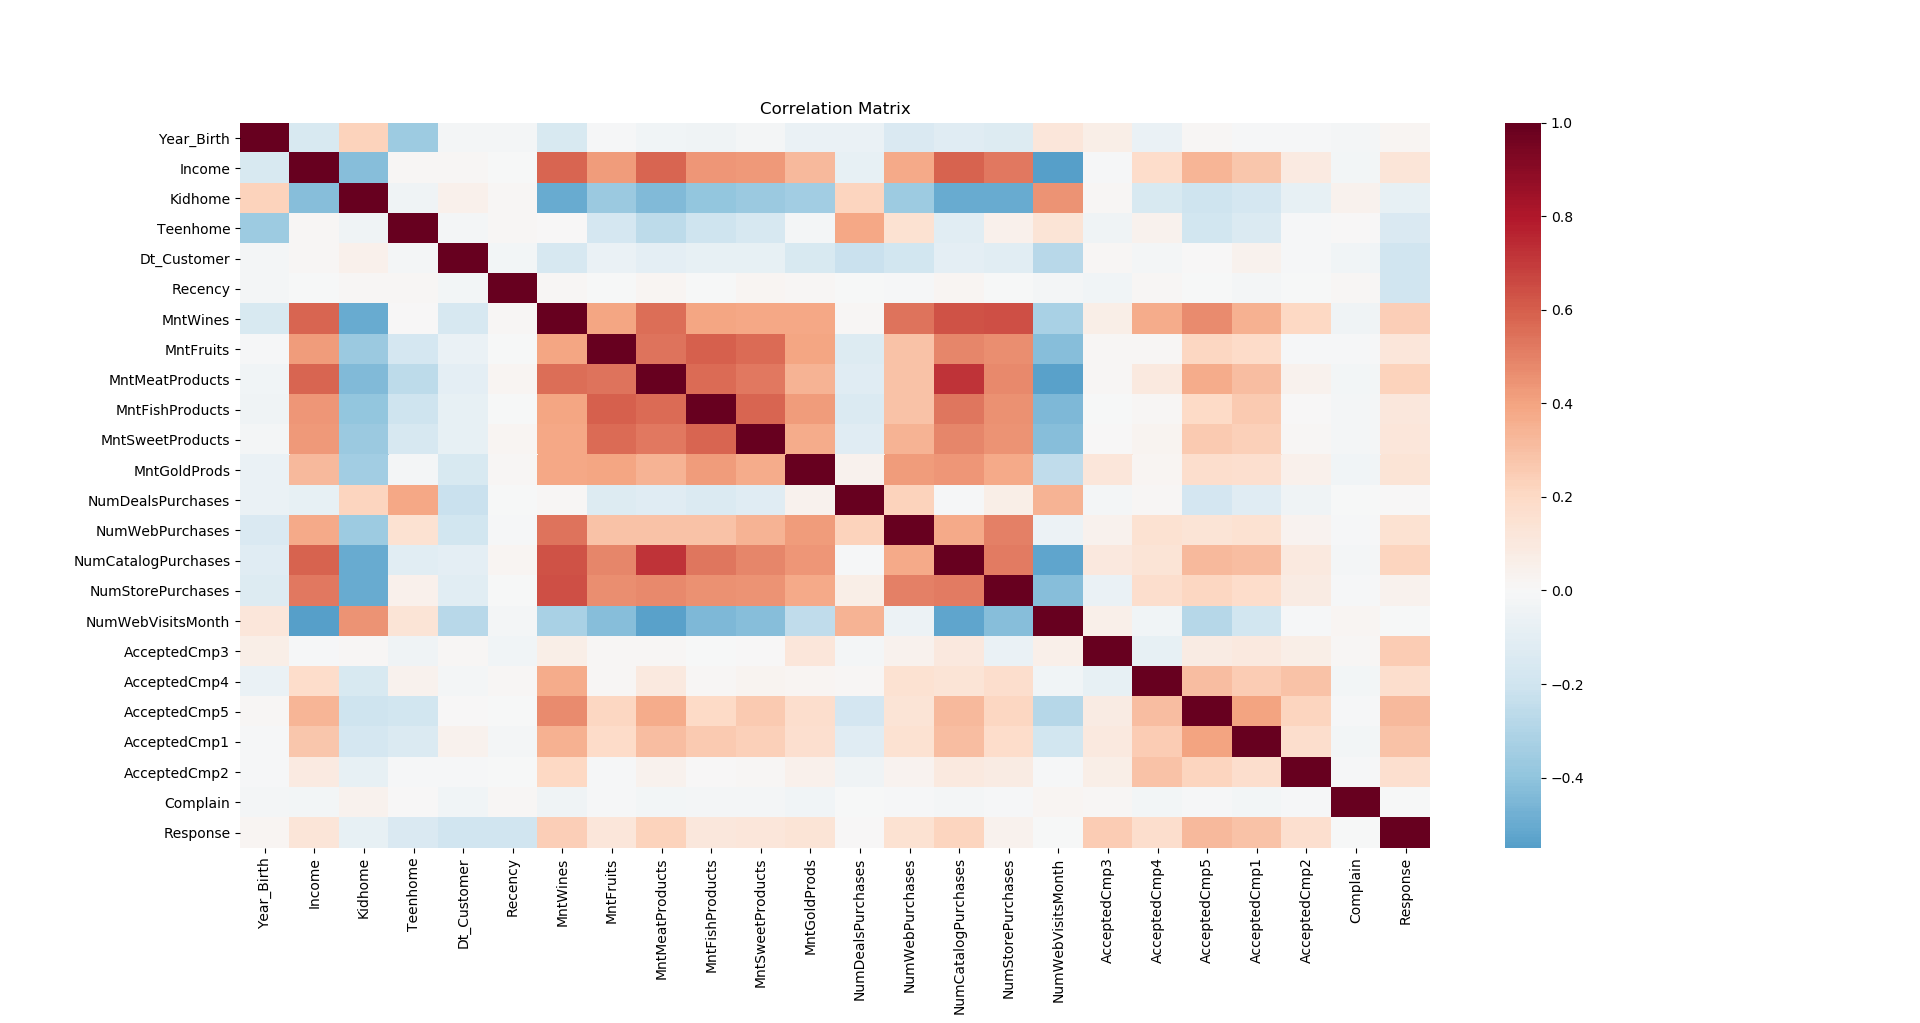
\includegraphics[scale=0.40]{Correlation_Matrix1.png}
\caption{Matrix of the correlation between features}
\end{figure}

As an example of something we can try to infer: from this matrix we can see a higher positive correlation between the amount of food products bought, which could imply that people buy many different product types everytime they shop.\\

Some interesting things we could try to extract from this are:
\begin{itemize}
\item Users who have a kid(s) at home have a lower income. The people who have a lower income buy less products (as expected). However, people who have kids or teenagers at home used more deals (maybe the user (parent) doens't trust the deals, but their children do?)
\item For some reason, users with higher income have a lower correlation with the number of webvisits per month (could be because they buy in bigger quantities, so they prefer to go to the store? Could be related to the fact that they buy more at once, so they don't access the website as often)
\item The item above could be supported by the fact that high income has a high correlation with web purchases.
\item Users who have children at home don't buy as much wine products (could be related to the income factor, since wine is rather expensive, but it could also be because some parents don't like drinking in front of their children.)
\item There is a higher correlation between accepting the campaigns, which could suggest that users who accept the campaigns are usually the same. However there is an almost null correlation between the acceptance of the 3rd campaign and the other features, which could suggest that people accepted it independently from the other campaings because it was a good offer, or just the opposite.
\item High income has a positive correlation with accepting the campaings. Since people with higher income buy more products, could it be that they are more willing to accept an offer to spend less?
\item There is a positive correlation between webvisits and deals purchases. Could it be that users see the deals when accessing the site, leading them to using the deals? Maybe the deals can only be found online.
\item We can see that the correlations between Response feature with the other features is similar to the previous campaings correlations. This could suggest that we can expect the users that have already accepted an offer in the past to accept this offer. The users who buy more quantities can also be expected to accept this offer.
\item For some reason, this campaing response has a higher negative correlation to recency than the previous campaigns. One possibility for this is some change in customer behaviour. Maybe users are coming back more often and seeing the offer?
\end{itemize}

There are many possibilities for what we could try to infer from these correlations, and it is hard to decide what is most likely to be correct, since correlation doesn't imply causation. However, at least we are able to see a pattern in the user base.\\

We could try to segment the user base on the following categories:
\begin{itemize}
\item[A]. Users with higher income, who buy a lot in less purchases, and are more prone to accepting an offer, since they spend more. They are less likely to have children and are usually older.
\item[B]. Users who have accepted previous campaing offers. These users buy big amounts and are more prone to accepting another offer. Directing these offers to these users who are more likely to accept them, could create a reliable user base.
\item[C]. Users who use the web more often, are younger and have lower income, like students, and buy less everytime they purchase something. These users are less likely to have children, since they are younger.
\item[D]. Users who have lower income, and more children at home, and make smaller purchases, but somewhat often. They are likely to make deal purchases, to spend less, or because they wouldn't be able to afford the products otherwise.
\end{itemize}

\section{User response to the campaing}

In this section we will make an analysis on the content of the tables, that can be found on the following archives: Categorical\_Info\_Response.csv, Binary\_Info\_Response.csv and Numeric\_Info\_Response.csv.

\section{Tables}\label{Tables}

\begin{table}[H]
\centering
\begin{tabular}{c|c|c|c|c|c|c|c|}
\cline{2-8}
                                          & mean     & std      & min  & 25\%     & 50\%    & 75\%     & max    \\ \hline
\multicolumn{1}{|c|}{Year\_Birth}         & 1968.84  & 11.83    & 1920 & 1959     & 1970    & 1977     & 1996   \\ \hline
\multicolumn{1}{|c|}{Income}              & 52247.25 & 25037.80 & 1730 & 35538.75 & 51741.5 & 68289.75 & 666666 \\ \hline
\multicolumn{1}{|c|}{Recency}             & 49.11    & 28.96    & 0    & 24       & 49      & 74       & 99     \\ \hline
\multicolumn{1}{|c|}{NumDealsPurchases}   & 2.33     & 1.93     & 0    & 1        & 2       & 3        & 15     \\ \hline
\multicolumn{1}{|c|}{NumWebPurchases}     & 4.08     & 2.78     & 0    & 2        & 4       & 6        & 27     \\ \hline
\multicolumn{1}{|c|}{NumCatalogPurchases} & 2.66     & 2.92     & 0    & 0        & 2       & 4        & 28     \\ \hline
\multicolumn{1}{|c|}{NumStorePurchases}   & 5.79     & 3.25     & 0    & 3        & 5       & 8        & 13     \\ \hline
\multicolumn{1}{|c|}{NumWebVisitsMonth}   & 5.32     & 2.43     & 0    & 3        & 6       & 7        & 20     \\ \hline
\end{tabular}
\caption{Summary information on some of the numerical features.}
\end{table}

\begin{table}[H]
\centering
\begin{tabular}{c|c|c|c|c|}
\cline{2-5}
                                   & count & unique & top   & freq \\ \hline
\multicolumn{1}{|c|}{Complain}     & 2240  & 2      & False & 2219 \\ \hline
\multicolumn{1}{|c|}{AcceptedCmp1} & 2240  & 2      & False & 2096 \\ \hline
\multicolumn{1}{|c|}{AcceptedCmp2} & 2240  & 2      & False & 2210 \\ \hline
\multicolumn{1}{|c|}{AcceptedCmp3} & 2240  & 2      & False & 2077 \\ \hline
\multicolumn{1}{|c|}{AcceptedCmp4} & 2240  & 2      & False & 2073 \\ \hline
\multicolumn{1}{|c|}{AcceptedCmp5} & 2240  & 2      & False & 2077 \\ \hline
\end{tabular}
\caption{Summary information on binary features.}
\end{table}

\begin{table}[H]
\centering
\begin{tabular}{l|l|l|l|l|}
\cline{2-5}
                                      & count & unique & top        & freq \\ \hline
\multicolumn{1}{|l|}{Education}       & 2240  & 5      & Graduation & 1127 \\ \hline
\multicolumn{1}{|l|}{Marital\_Status} & 2240  & 4      & Married    & 1446 \\ \hline
\end{tabular}
\caption{Summary data on categorical features}
\end{table}

\section{Dataset Vizualization with PCA}\label{PCA}

\begin{figure}[H]
\centering
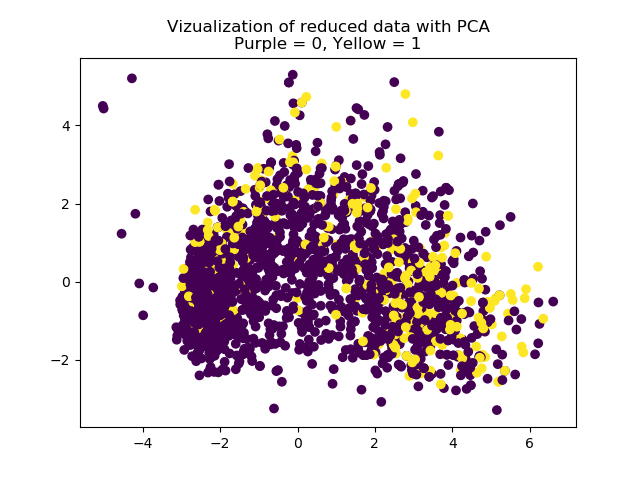
\includegraphics[scale=0.75]{PCA1.png}
\caption{The data was reduced with PCA to 2D for vizualization. The data was scalled with a Standard scaler.}
\end{figure}

\begin{figure}[H]
\centering
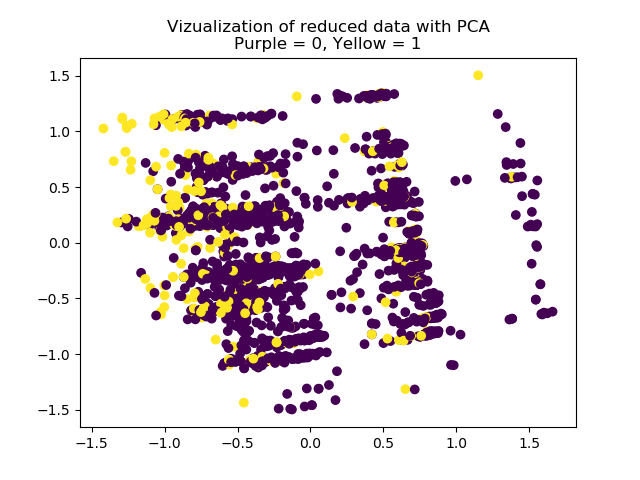
\includegraphics[scale=0.75]{PCA2.png}
\caption{The data was reduced with PCA to 2D for vizualization. The data was scalled with a MinMax scaler.}
\end{figure}

\end{document}























